
%(BEGIN_QUESTION)
% Copyright 2006, Tony R. Kuphaldt, released under the Creative Commons Attribution License (v 1.0)
% This means you may do almost anything with this work of mine, so long as you give me proper credit

A {\it tank expert} system uses three pressure transmitters to measure level and density of a liquid in a large storage vessel.  The three transmitters are labeled ``top,'' ``middle,'' and ``bottom,'' as such:

$$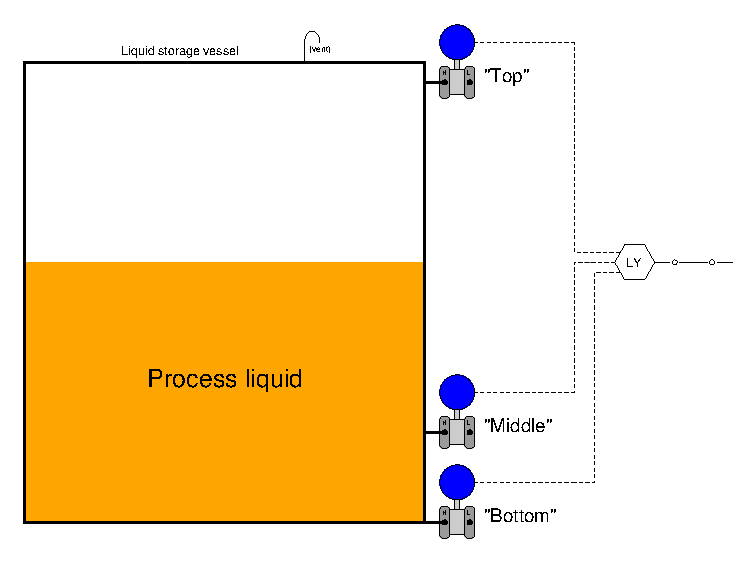
\includegraphics[width=15.5cm]{i00254x01.eps}$$

Tank expert systems use a computer (LY in the diagram) to process data gathered from the three pressure transmitters, calculating both liquid density and liquid level.  The distance between the ``middle'' and ``bottom'' pressure transmitters is known from installation and entered into this computer system as a constant value, to be used in the calculations.  An important requirement of a tank expert system is that the liquid level must be above the ``middle'' pressure transmitter's location if density is to be calculated.

Suppose that a tank expert system has the ``middle'' transmitter located 10 feet above the bottom of the vessel, the ``bottom'' transmitter at the very bottom of the vessel, and the ``top'' transmitter at the very top.  Supposing that the vessel is vented at the top (preventing any vapor pressure buildup) and is 40 feet tall, and the liquid level inside is 15 feet with a specific gravity of 0.86, what pressures will the three pressure transmitters report to the computer system under these conditions?  In other words, what will be the ``raw'' data input to the computer system under these conditions?

\underbar{file i00254}
%(END_QUESTION)





%(BEGIN_ANSWER)

``Top'' pressure = 0 "W.C.

``Middle'' pressure = 51.6 "W.C.

``Bottom'' pressure = 154.8 "W.C.

%(END_ANSWER)





%(BEGIN_NOTES)


%INDEX% Measurement, level: hydrostatic pressure
%INDEX% Measurement, level: tank expert system

%(END_NOTES)


